\documentclass[tikz,border=2pt]{standalone}

\usepackage{tikz}
\usepackage{tikz-qtree}

\begin{document}

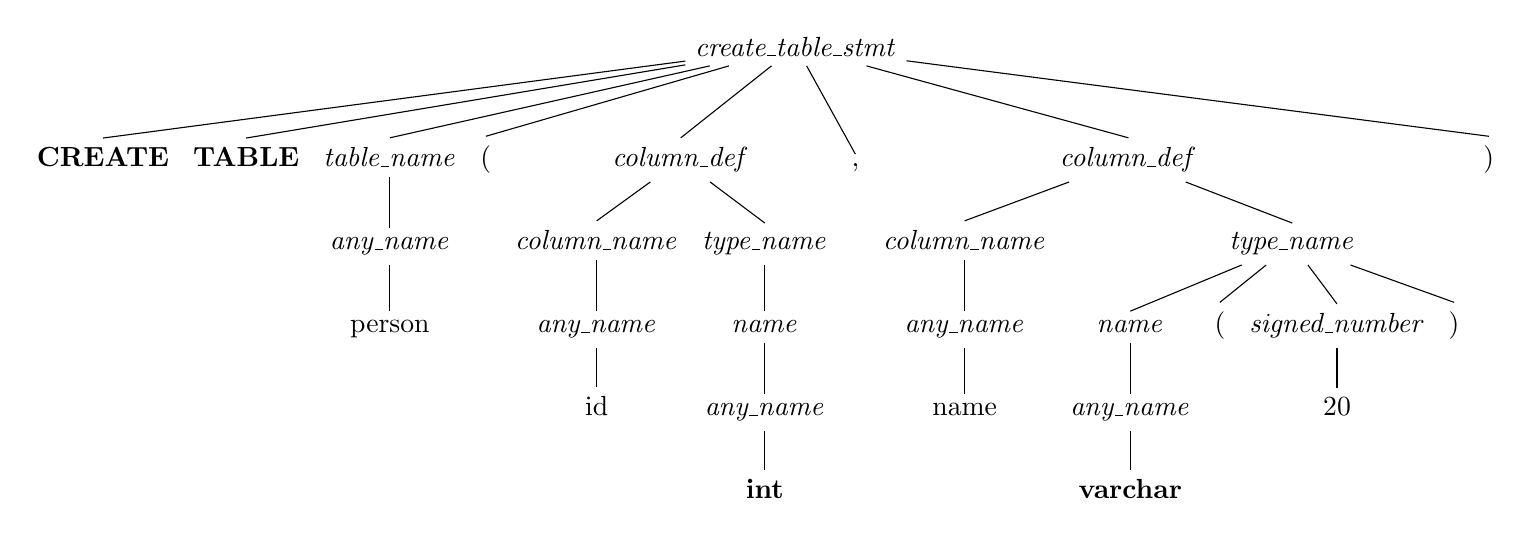
\begin{tikzpicture}
    \tikzset{
        level 1/.style={level distance=4em},
        edge from parent path={(\tikzparentnode) -- (\tikzchildnode.north)}
    }
    \Tree [.\textit{create\_table\_stmt}
            \textbf{CREATE}
            \textbf{TABLE}
            [.\textit{table\_name} [.\textit{any\_name} person ] ]
            (
            [.\textit{column\_def}
                [.\textit{column\_name} [.\textit{any\_name} id ] ]
                [.\textit{type\_name} [.\textit{name} [.\textit{any\_name} \textbf{int} ] ] ]
            ]
            ,
            [.\textit{column\_def}
                [.\textit{column\_name} [.\textit{any\_name} name ] ]
                [.\textit{type\_name} [.\textit{name} [.\textit{any\_name} \textbf{varchar} ] ] ( [.\textit{signed\_number} 20 ] ) ]
            ]
            )
          ]
\end{tikzpicture}

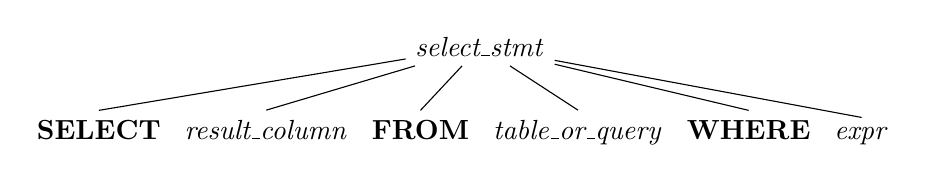
\begin{tikzpicture}
    \tikzset{
        % level 1/.style={level distance=3em,sibling distance=.6em},
        edge from parent path={(\tikzparentnode) -- (\tikzchildnode.north)}
    }
    \Tree [.\textit{select\_stmt}
            \textbf{SELECT}
           \textit{result\_column}
            \textbf{FROM}
            \textit{table\_or\_query}
            \textbf{WHERE}
            \textit{expr}
          ]
\end{tikzpicture}

\end{document}
